\section{Demografis indflydelse på vurderinger}
\label{sec:Demografi}
%
***NOTER***

I dette afsnit beskrives hvordan forskellene mellem mennesker kan være med til at påvirke vurderingerne af robotten. Der kigges isoleret på hvordan de demografiske faktorer påvirker hver enkelt skala. Det er valgt kun at medtage de plots hvor der ses en tendens, men analysen er lavet på tværs af alle demografiske faktorer og alle skalaer, med undtagelse af hvor ofte folk rejser.


Der var en lille korrelation mellem folks aldre og om de syntes at den kørte for hurtigt \autoref{fig:age6}.

\begin{figure}[H]
\centering
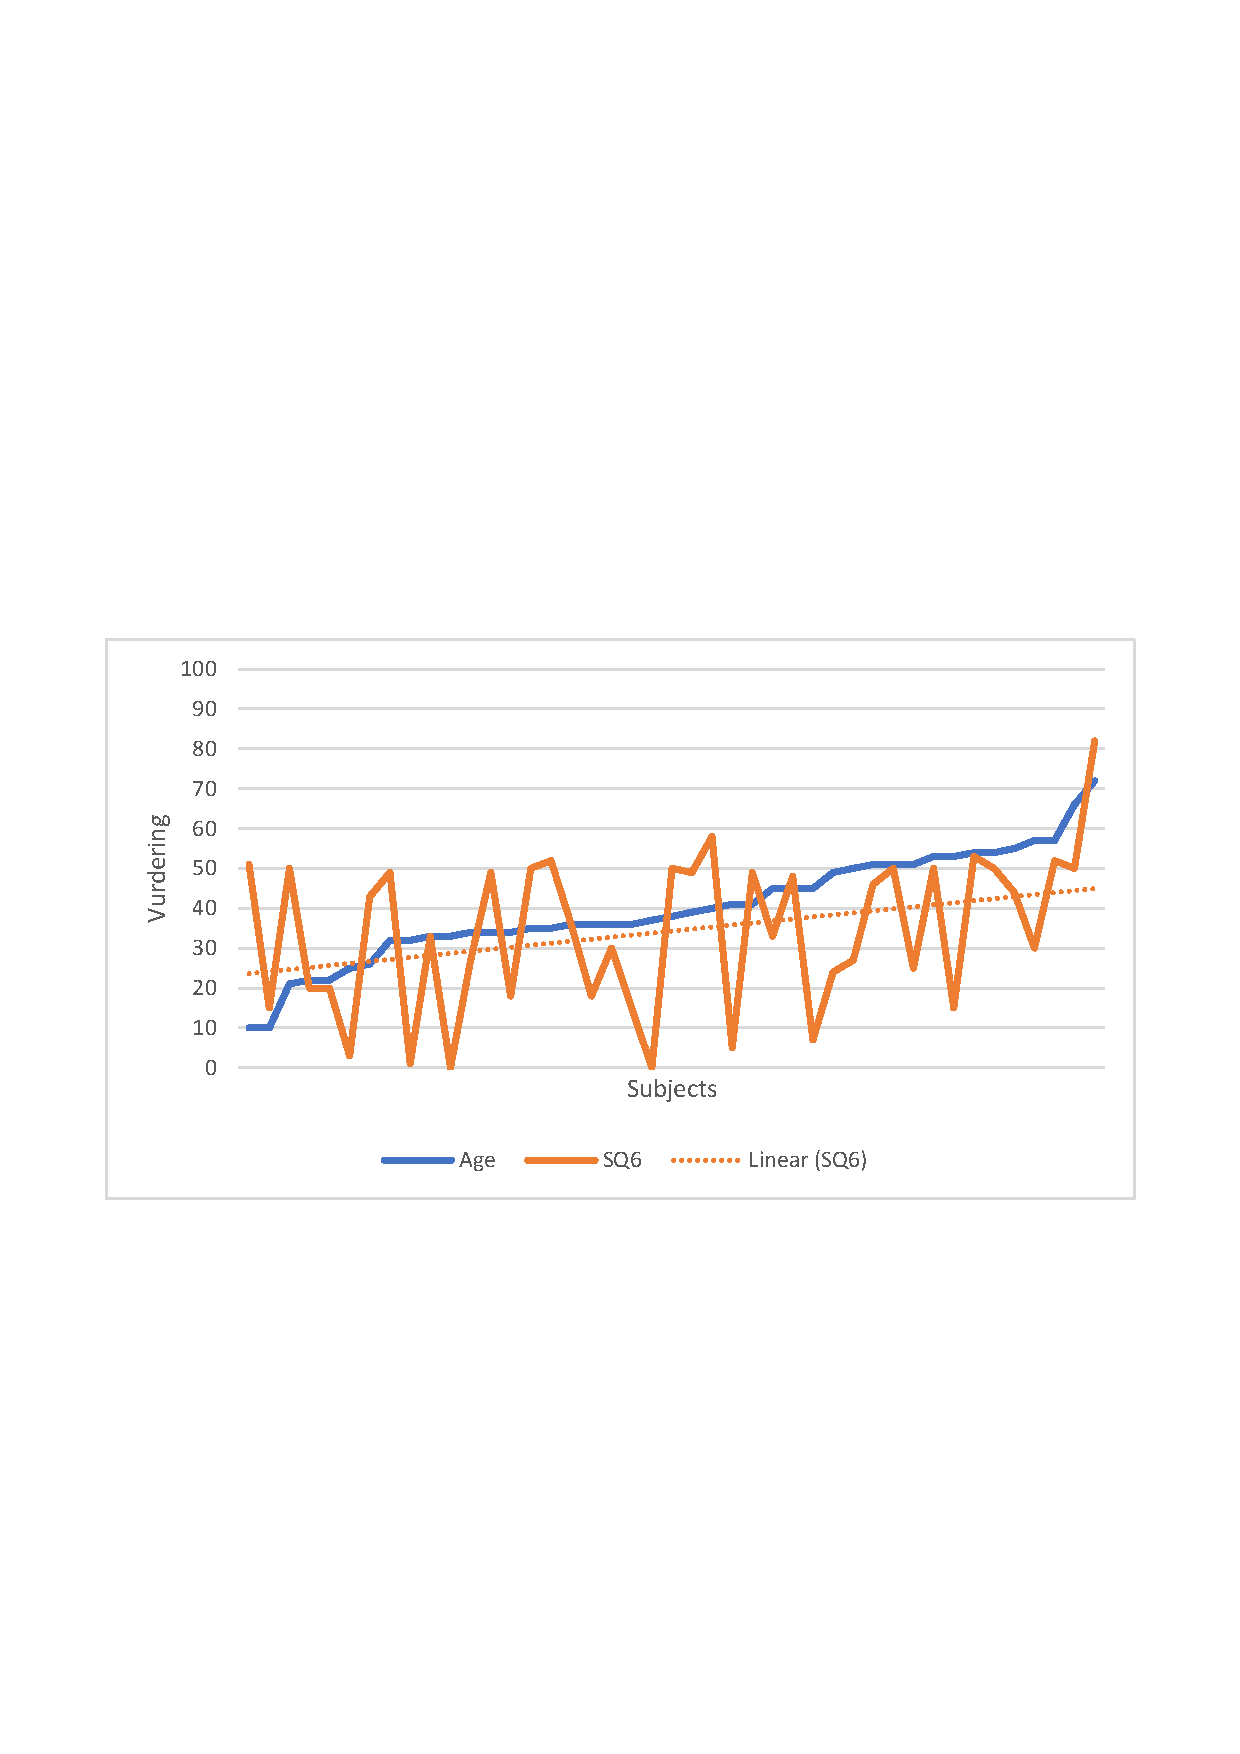
\includegraphics[width=\textwidth]{Figure/DatabehandlingSkalaer/Demografi/age6.pdf}
\caption{}
\label{fig:age6}
\end{figure}
\noindent

Der var en negativ korrelation mellem hvor gamle de var og hvor sjov og spændende de synes den var. 

\begin{figure}[H]
\centering
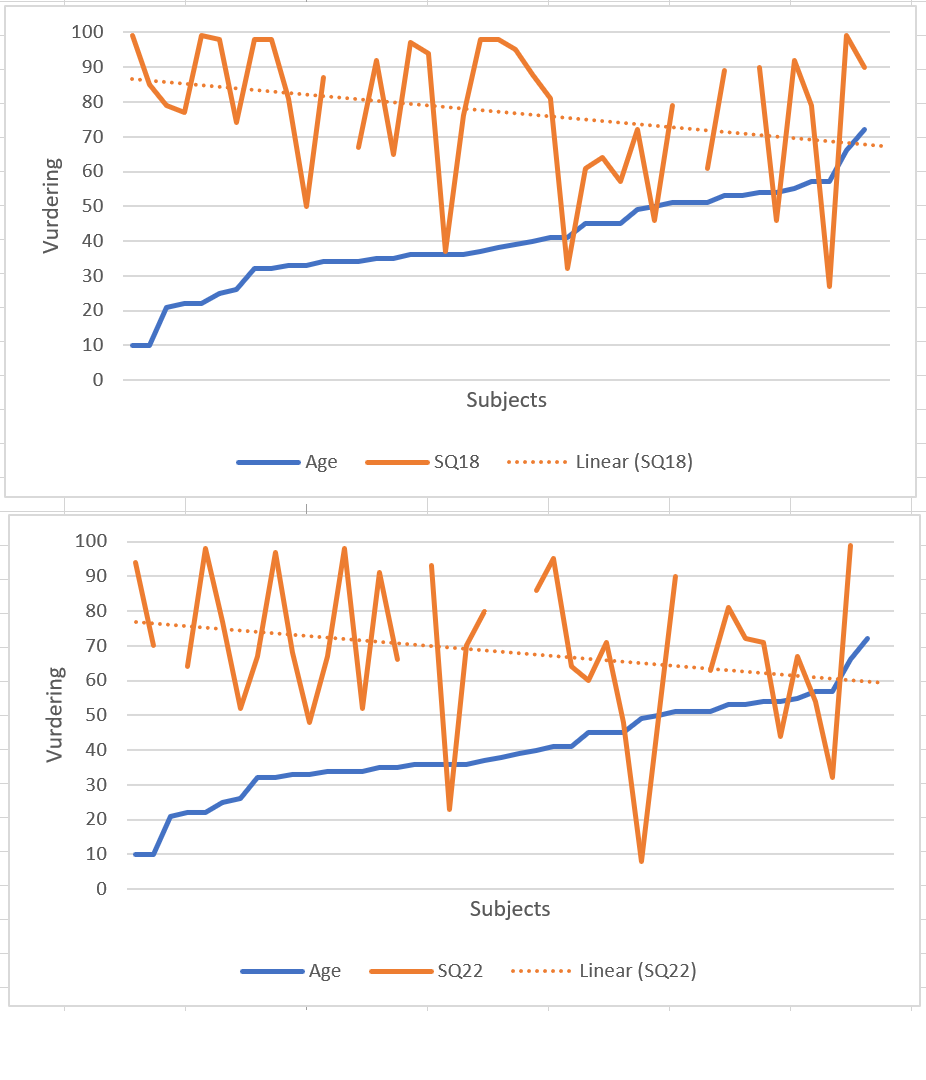
\includegraphics[width=\textwidth]{Figure/DatabehandlingSkalaer/Demografi/age18_22.png}
\caption{}
\label{fig:age18_22}
\end{figure}
\noindent

\fxnote{Passer muligvis bedre ind under robothøjde} Vi kan se at jo større højdeforskellen er mellem menneske og robot, jo sødere og mere elegant opleves robotten. \autoref{fig:heightRatio19}. Det betyder altså at en robotten opleves sødere og mere elegant, jo lavere den er i forhold til brugeren, da de fleste testpersoner var højere end robotten.

\begin{figure}[H]
\centering
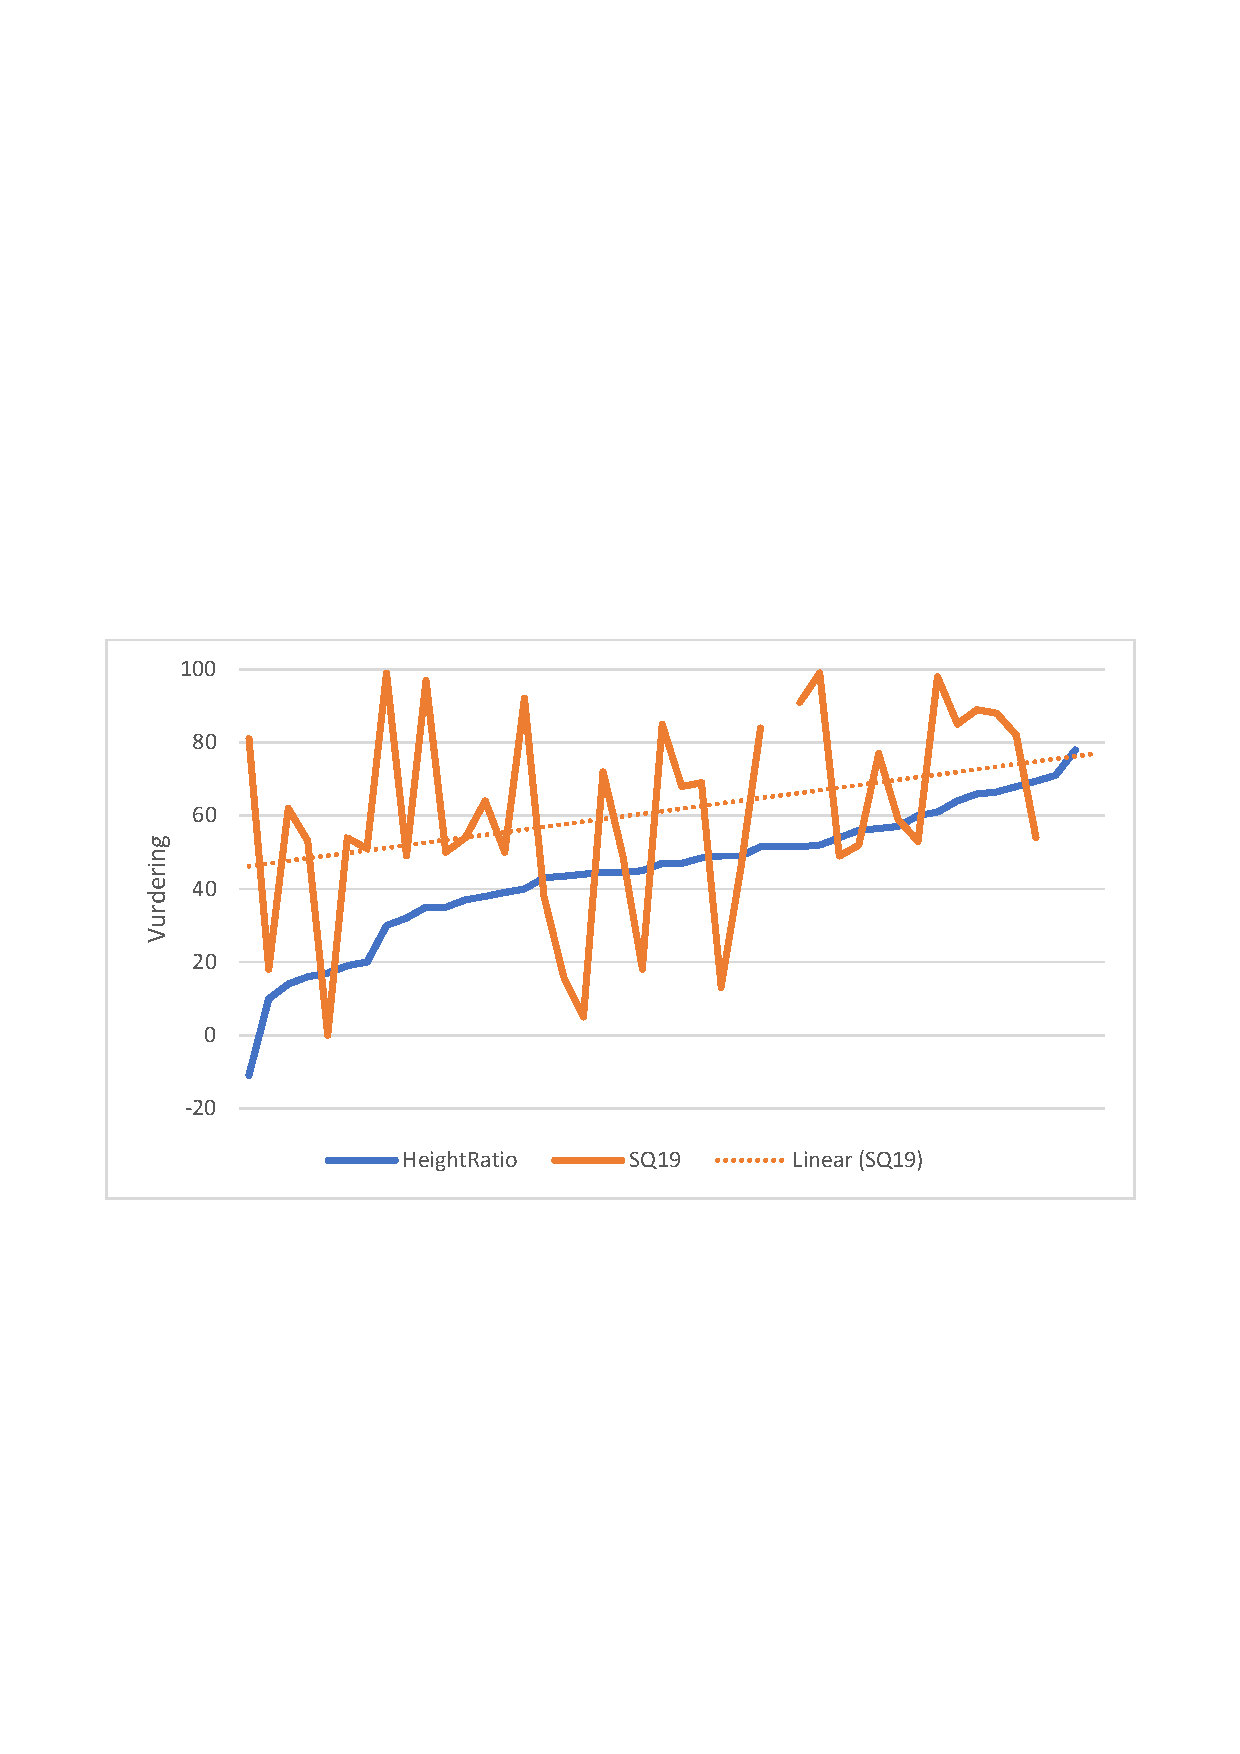
\includegraphics[width=\textwidth]{Figure/DatabehandlingSkalaer/Demografi/HeightRatio.pdf}
\caption{}
\label{fig:heightRatio19}
\end{figure}
\noindent

Robotten opleves også hurtigere og vildere, når den er lav, hvilket giver god mening, da robotten rent faktisk kører hurtigere ved de lave højder \autoref{fig:heightRatio4_6}.


\begin{figure}[H]
\centering
\includegraphics[width=\textwidth]{Figure/DatabehandlingSkalaer/Demografi/HeightRatio4_6.png}
\caption{}
\label{fig:heightRatio4_6}
\end{figure}
\noindent


Der var meget stor forskel på hvor godt skærmen reagerede, og der var ikke nogle af faktorerne som beskrev hvad denne forskel kom af. For eksempel var dem som var glade for teknologi ikke bedre til at trykke rigtigt på skærmen.

Vi kan se at der er svaret lige omkring midten for spørgsmål 5 og 7 på tværs af alle de demografiske faktorer. 5 og 7 er derfor ikke særligt beskrivende for den oplevelse folk har haft, da alle har svaret cirka det samme både på tværs af demografi og på tværs af de stimuli de har været udsat for (forskellige højder, afstande og vinkler). 5=robotten er for tæt på/langt væk, 7=robotten er for høj/lav.